\documentclass[a4paper,12pt]{article}

%%% Работа с русским языком % для pdfLatex
\usepackage{cmap}					% поиск в~PDF
\usepackage{mathtext} 				% русские буквы в~фомулах
\usepackage[T2A]{fontenc}			% кодировка
\usepackage[utf8]{inputenc}			% кодировка исходного текста
\usepackage[russian]{babel}	% локализация и переносы
\usepackage{indentfirst} 			% отступ 1 абзаца
\usepackage{amsmath}
%%% Работа с русским языком % для XeLatex
%\usepackage[english,russian]{babel}   %% загружает пакет многоязыковой вёрстки
%\usepackage{fontspec}      %% подготавливает загрузку шрифтов Open Type, True Type и др.
%\defaultfontfeatures{Ligatures={TeX},Renderer=Basic}  %% свойства шрифтов по умолчанию
%\setmainfont[Ligatures={TeX,Historic}]{Times New Roman} %% задаёт основной шрифт документа
%\setsansfont{Comic Sans MS}                    %% задаёт шрифт без засечек
%\setmonofont{Courier New}
%\usepackage{indentfirst}
%\frenchspacing

%%% Дополнительная работа с математикой
\usepackage{amsfonts,amssymb,amsthm,mathtools}
\usepackage{amsmath}
\usepackage{icomma} % "Умная" запятая: $0,2$~--- число, $0, 2$~--- перечисление
\usepackage{upgreek}

%%% Страница
\usepackage{extsizes} % Возможность сделать 14-й шрифт

%% Шрифты
\usepackage{euscript}	 % Шрифт Евклид
\usepackage{mathrsfs} % Красивый матшрифт

%% Свои команды
\DeclareMathOperator{\sgn}{\mathop{sgn}} % создание новой конанды \sgn (типо как \sin)
\usepackage{csquotes} % ещё одна штука для цитат
\newcommand{\pd}[2]{\ensuremath{\cfrac{\partial #1}{\partial #2}}} % частная производная
\newcommand{\abs}[1]{\ensuremath{\left|#1\right|}} % модуль
\renewcommand{\phi}{\ensuremath{\varphi}} % греческая фи
\newcommand{\pogk}[1]{\!\left(\cfrac{\sigma_{#1}}{#1}\right)^{\!\!\!2}\!} % для выражений для погрешности

% Ссылки
\usepackage{color} % подключить пакет color
% выбрать цвета
\definecolor{BlueGreen}{RGB}{49,152,255}
\definecolor{Violet}{RGB}{120,80,120}
% назначить цвета при подключении hyperref
\usepackage[unicode, colorlinks, urlcolor=blue, linkcolor=blue, pagecolor=blue, citecolor=blue]{hyperref} %синие ссылки
%\usepackage[unicode, colorlinks, urlcolor=black, linkcolor=black, pagecolor=black, citecolor=black]{hyperref} % для печати (отключить верхний!)
\mathtoolsset{showonlyrefs=true} % Показывать номера только у тех формул, на которые есть \eqref{} в~тексте.


%% Перенос знаков в~формулах (по Львовскому)
\newcommand*{\hm}[1]{#1\nobreak\discretionary{}
	{\hbox{$\mathsurround=0pt #1$}}{}}

%%% Работа с картинками
\usepackage{graphicx}  % Для вставки рисунков
\graphicspath{{images/}{images2/}}  % папки с картинками
\setlength\fboxsep{3pt} % Отступ рамки \fbox{} от рисунка
\setlength\fboxrule{1pt} % Толщина линий рамки \fbox{}
\usepackage{wrapfig} % Обтекание рисунков и таблиц текстом
\usepackage{multicol}

%%% Работа с таблицами
\usepackage{array,tabularx,tabulary,booktabs} % Дополнительная работа с таблицами
\usepackage{longtable}  % Длинные таблицы
\usepackage{multirow} % Слияние строк в~таблице
\usepackage{caption}
\captionsetup{labelsep=period, labelfont=bf}

%%% Оформление
\usepackage{indentfirst} % Красная строка
%\setlength{\parskip}{0.3cm} % отступы между абзацами


%%% Правильные мат. символы для русского языка
\renewcommand{\epsilon}{\ensuremath{\varepsilon}}
\renewcommand{\phi}{\ensuremath{\varphi}}
\renewcommand{\kappa}{\ensuremath{\varkappa}}
\renewcommand{\le}{\ensuremath{\leqslant}}
\renewcommand{\leq}{\ensuremath{\leqslant}}
\renewcommand{\ge}{\ensuremath{\geqslant}}
\renewcommand{\geq}{\ensuremath{\geqslant}}
\renewcommand{\emptyset}{\varnothing}

%%% Название разделов
\usepackage{titlesec}
\titlelabel{\thetitle.\quad}

\title{}
\author{Ксения Зайцева}
\date{}
\usepackage[left=1.27cm,right=1.27cm,top=1.27cm,bottom=2cm]{geometry}

\RequirePackage{caption}
\DeclareCaptionLabelSeparator{defffis}{ — }
\captionsetup{justification=centering,labelsep=defffis}

\begin{document} 

\renewcommand{\figurename}{\textbf{Рисунок}}		%Чтобы вместо figure под рисунками писал "рис"
\renewcommand{\tablename}{\textbf{Таблица}}		%Чтобы вместо table над таблицами писал Таблица

\begin{titlepage}
\begin{center} 
 
\large Московский физико-технический институт\\
Физтех-школа биологической и медицинской физики\\
\vspace{7cm}
{\huge
\begin{center}
    {Лабораторная работа по физическим методам исследований}\\
    {\bf  Основы флуоресцентной спектроскопии	}
\end{center}
}
\end{center}
\begin{flushright}
{\LARGE Авторы:\\ Фитэль Алёна, Б06-103\\ Попеску Полина, Б06-103 \\ }

\end{flushright}

\begin{center}
\vfill Долгопрудный 2024
\end{center}
\end{titlepage}

\newpage
\setcounter{page}{2}


\section*{Теоретическая часть}
\subsection*{Люминесценция и флуоресценция}
Способностью излучать электромагнитные волны (в том числе и видимого диапазона)
обладают все вещества. Эта способность обусловлена преобразованием внутренней энергии
в энергию электромагнитного поля. Такой тип излучения называют тепловым и спектр этого
излучения, как правило, сплошной, а частота, на которой излучение имеет максимальную
интенсивность, зависит от температуры тела.
Среди всех веществ можно выделить группу соединений, особым свойством которых
является способность испускать излучение, возбуждаемое каким-либо источником энергии и
не обусловленное нагреванием веществ. Это излучение, продолжающееся в течение времени,
значительно превышающего период световых колебаний, называют люминесценцией.
Вещества, способные люминесцировать, называются люминофорами.

Физическая природа люминесценции состоит в излучательных переходах электронов атомов
или молекул из возбуждённого состояния в основное. Обычно энергии электронных,
колебательных и вращательных уровней связаны соотношением 
\begin{equation}
    E_\text{эл} \gg E_\text{кол} \gg E_\text{вр},
\end{equation}
тогда внутреннюю энергию молекулы можно представить суммой (приближение Борна-Оппенгеймера):
\begin{equation}
    E = E_\text{эл} + E_\text{кол} + E_\text{вр}.
\end{equation}

Энергии молекулы могут изменяться только дискретно, при этом разность энергий $\Delta E$ между двумя ближайшими энергетическими состояниями определяется
уравнением:
\begin{equation}
    \Delta E = \Delta E_\text{эл} + \Delta E_\text{кол} + \Delta E_\text{вр}.
\end{equation}
Энергетические состояния молекулы и возможные электронные переходы могут быть представлены в виде схемы уровней энергии – диаграммы Ябло́нского, где каждый
электронный уровень расщепляется на ряд колебательных подуровней, а каждый
колебательный – на ряд вращательных подуровней. На этой диаграмме буквами $S_0,
S_1, S_2$ обозначены синглетные состояния молекулы. При этом суммарный спин S всех
электронов молекулы равен 0, в результате мультиплетность молекулы М = 2S + 1= 1. Если
суммарный спин молекулы S = 1 и мультиплетность М = 2S + 1 = 3, то молекула находится в
триплетном состоянии. Триплетные состояния обозначаются буквами $T_1$, $T_2$ и т.д. 
\begin{figure}
    \centering
    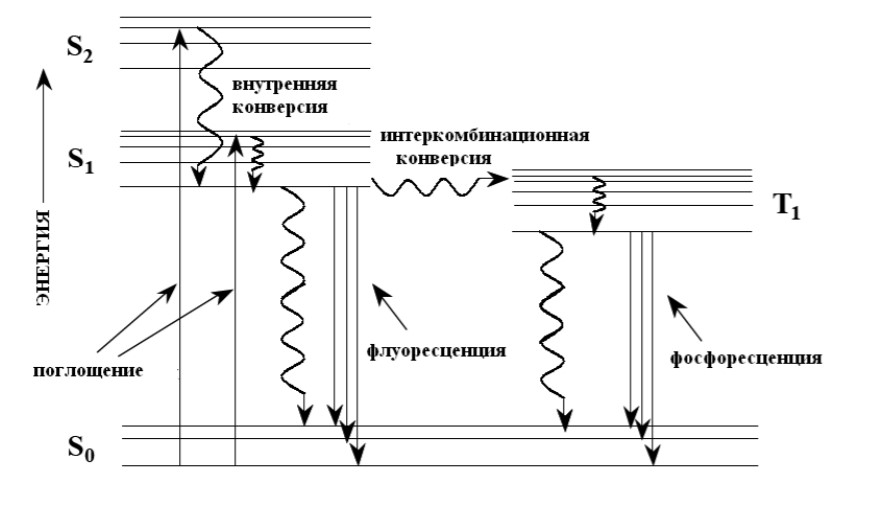
\includegraphics[scale=0.8]{yabl.jpg}
    \caption{Диаграмма Яблонского}
\end{figure}
\\
Наиболее вероятными энергетическими переходами являются переходы без
изменения мультиплетности (например, cинглет - синглетный переход при
поглощении кванта возбуждения и обратный ему переход при дезактивации
молекулы). Излучательный переход между двумя состояниями одинаковой мультиплетности
называется флуоресценцией. Типичное время жизни такого возбужденного состояния
составляет $10^{-11}-10^{-8}$ с.
\\
Излучательный переход между состояниями разной мультиплетности называется
фосфоресценцией. Переходы между уровнями с различной мультиплетностью являются
запрещенными с точки зрения квантовой механики, поэтому время жизни возбужденного
состояния при фосфоресценции значительно больше, чем при флуоресценции, и составляет
$10^{-4}-10^{-2}$ с.
\\
За счет длительного времени жизни триплетного состояния, молекулы, пребывающие
в нем, легко теряют свою энергию в различных безызлучательных процессах. Такие
процессы могут протекать как внутри отдельной молекулы, так и в результате
межмолекулярного взаимодействия. 
\\
К внутримолекулярным безызлучательным переходам относится внутренняя и
интеркомбинационная конверсия. В первом случае переход происходит между
состояниями одинаковой, а во втором - разной мультиплетности.

\subsection*{Законы флуоресценции}
В многоатомных молекулах спектр испускания сдвинут относительно спектра
возбуждения в длинноволновую область. Сдвиг между
положением максимумов спектра поглощения и флуоресценции называется стоксовым
сдвигом, а указанное выше правило – законом Стокса. 
Также спектры испускания и возбуждения флуоресценции, как правило, зеркально
симметричны относительно прямой, проходящей через точку их пересечения
перпендикулярно оси длин волн. Это правило получило название правила Левшина
(правило зеркальной симметрии). Оно обусловлено сходством распределения колебательных
подуровней по энергиям у основного и возбужденного состояний. В некоторых случаях
наблюдаются отклонения от правила зеркальной симметрии, вызванные геометрическими
перегруппировками в молекуле или реакциями в возбужденном состоянии. 
\begin{figure}
    \centering
    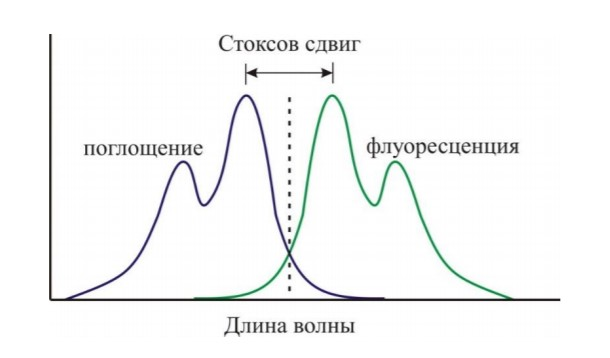
\includegraphics[scale=0.9]{stoks.jpg}
    \caption{Стоксов сдвиг и правило Левшина}
\end{figure}

По принципу Франка-Кондона переходы электронов при поглощении энергии молекулой и при ее
излучении – вертикальные. Согласно правилу Каши, излучение фотона (флуоресценция и
фосфоресценция) происходит только с низшего возбужденного электронного состояния
молекулы. Правило Каши необходимо учитывать для понимания спектров излучения
возбужденной молекулы (форма и положение спектра флуоресценции не зависят от длины
волны возбуждающего света). При поглощении фотона молекула, находящаяся в основном
состоянии, переходит в одно из возбужденных состояний, имеющих большую энергию. Однако, в соответствии с эмпирическим правилом Каши, излучение фотона (в
случае флуоресценции — это переход между синглетными состояниями) происходит
только с нижнего колебательного уровня возбужденного электронного состояния.
\\
Для оценки интенсивности фотолюминесценции обычно используется относительная
(безразмерная) величина, называемая \textbf{квантовым выходом} $\phi$. Этот параметр определяется
как отношение числа испущенных квантов $n_F$ к числу поглощенных квантов $n_A$:
\begin{equation}
    \phi = \frac{n_F}{n_A}.
\end{equation}

Чем больше квантовый выход, тем эффективнее преобразование возбуждающего
света в излучение флуоресценции.

С.И.Вавилов сформулировал закон для квантового выхода: квантовый выход не
зависит от длины волны возбуждения, если выполняется закон Стокса, т.е. если длина волны
возбуждающего света ($\lambda_{ex}$) меньше длины волны флуоресценции ($\lambda_F$). Из закона Вавилова
следует, что в определенном спектральном диапазоне
спектр флуоресценции не зависит от длины волны возбуждающего излучения.
\subsection*{Тушение флуоресценции}
Тушением флуоресценции называют любые процессы, которые
уменьшают интенсивность флуоресценции данного вещества. К тушению может проводить
множество процессов, в том числе реакции в возбужденном состоянии, перенос энергии,
образование комплексов и тушение при столкновениях. В данной работе исследуются два
процесса – тушение, связанное со случайными столкновениями между флуорофором и
гасителем (тушителем), которое называется динамическим, и тушение, обусловленное
образованием нефлуоресцирующего комплекса между флуорофором и гасителем –
статическое тушение. Для тушения (и статического, и динамического) требуется контакт
между молекулами флуорофора и гасителя. Гаситель должен диффундировать к флуорофору
в течение времени нахождения последнего в возбужденном состоянии. В результате
контакта флуорофор возвращается в основное состояние без излучения фотона.

Для динамического тушения флуоресценции реакция взаимодействия флуорофора и
гасителя имеет вид:
\begin{equation}
    M^* + Q \rightarrow M + Q; \quad w = k_q [M^*][Q].
\end{equation}
Здесь $M^*$ и $M$ - концентрации флуорофора в возбужденном и невозбужденном состоянии, Q - гаситель.

Эта реакция описывается уравнением \textbf{Штерна-Фальмера}:
\begin{equation}
    \frac{F_0}{F} = 1 + K_q \tau_0 [Q] = 1 + K_\text{дин}[Q]
\end{equation}
где $F_0$, F – интенсивность флуоресценции в отсутствие и в присутствии гасителя
соответственно, $\tau_0$ – время затухания флуоресценции в отсутствии гасителя, [Q] –
концентрация гасителя, $K_\text{дин} = K_q \tau_0$ – штерн-фольмеровская константа тушения. Данные по
тушению обычно представляют в координатах $\frac{F_0}{F}$ от [Q]. График отсекает отрезок на оси
$\frac{F_0}{F}$, равный 1, и имеет наклон, равный $K_\text{дин}$. 
Динамическое тушение можно рассматривать как один из процессов
безызлучательной дезактивации возбужденного состояния флуоресцирующей молекулы,
приводящей к уменьшению его времени жизни. В этом случае можно строго показать, что
динамическое тушение приводит к одинаковому уменьшению интенсивности и времени
затухания флуоресценции:
\begin{equation}
    \frac{F_0}{F} = \frac{\tau_0}{\tau}
\end{equation}

В этой работе в качестве гасителя динамического типа используются ионы йода.
Известно, что тяжелые галогены, такие как йод и бром- увеличивают константу
интеркомбинационной конверсии в триплетное состояние из-за спин-орбитального
взаимодействия, возбужденного в синглетном состоянии флуорофора и галогена. Так как
время жизни в триплетном состоянии относительно большое, то такое состояние сильно
тушится другими процессами.
Частота столкновений флуорофора с гасителем дается выражением:
\begin{equation}
    Z = K_0 [Q],
\end{equation}
где $K_0$ – диффузионно-контролируемая (скорость реакции лимитируется сближением частиц
в результате диффузии) бимолекулярная константа скорости, которая может быть
вычислена по уравнению Смолуховского:
\begin{equation}
   K_o = 4 \pi R_{\sum} D_{\sum} N_A.
\end{equation}
Как уже отмечалось, \textbf{статическое тушение} происходит в результате образования
флуоресцирующего комплекса MQ в основном состоянии между флуорофором M и
гасителем Q. Как только произошло поглощение света, комплекс медленно
возвращается в основное состояние без испускания фотона.

Легко получить выражение для константы ассоциации комплекса:
\begin{equation}
    K_\text{ст} = \frac{[MQ]}{[M][Q]};
\end{equation}
Тогда 
\begin{equation}
    \frac{F_0}{F} = 1 + K_\text{ст}[Q].
\end{equation}
Видно, что зависимость $\frac{F_0}{F}$ от [Q] идентична зависимости, получаемой для
динамического тушения, за исключением того, что константа скорости тушения здесь
заменяется константой ассоциации.
В данной работе в качестве статического гасителя используются сами молекулы
родамина, т.к. при увеличении его концентрации начинают образовываться димеры, которые
не флуоресцируют.

\begin{figure}[h!]
\center{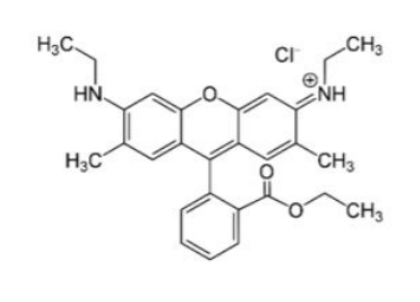
\includegraphics[scale=0.8]{Screenshot 2024-04-04 at 14.13.12.png}}
\caption{Структура родамина 6G}
\end{figure}


\newpage
\section*{Ход работы и обработка результатов}

\begin{enumerate}
    \subsection*{Задание 1. Исследование зависимости спектров поглощения и флуоресценции растворов родамина 6G от концентрации}

\item Приготовим водные растворы родамина 6G различных концентраций. Снимем спектры флуоресцентрии растворов различной концентрации.
\begin{figure}[h!]
\center{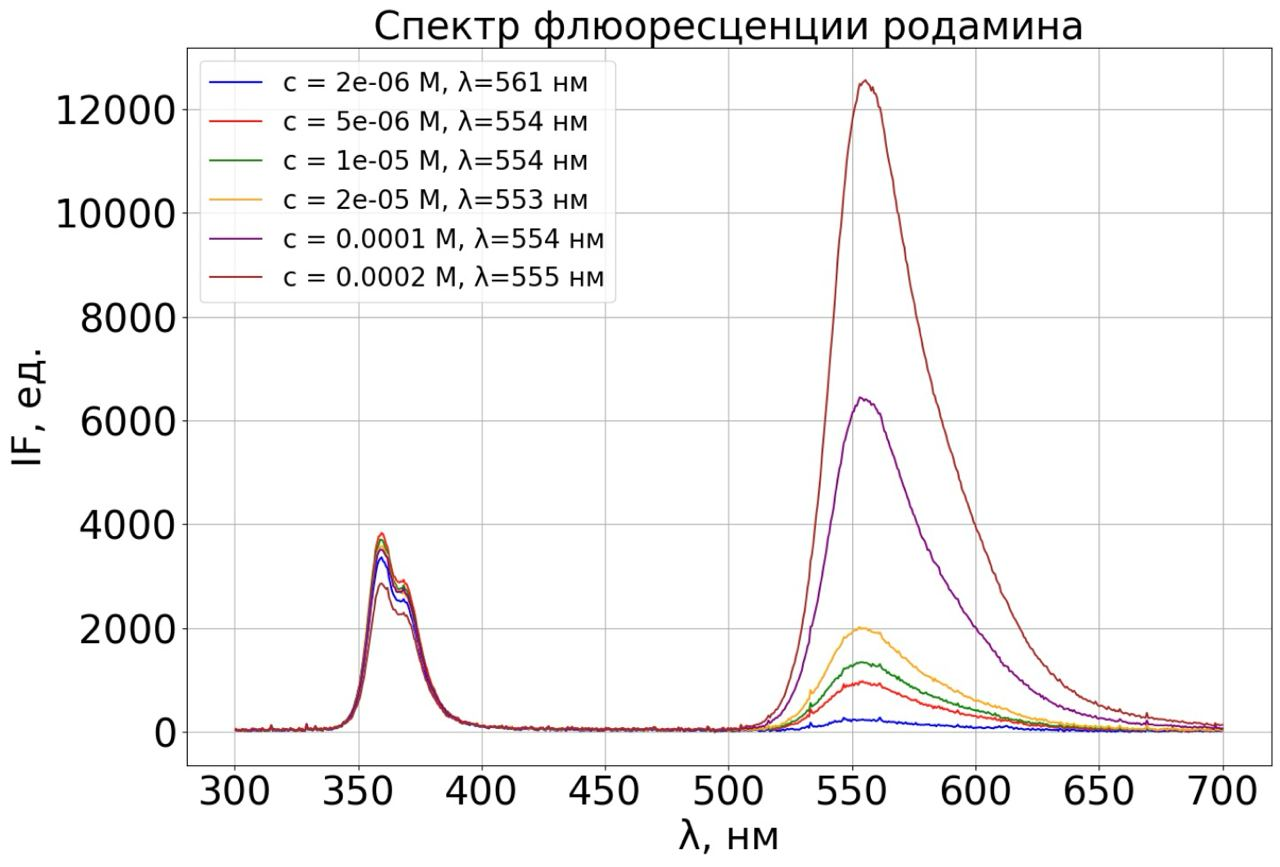
\includegraphics[scale=0.3]{fluor_spectr.jpeg}}
\caption{Флуоресценция родамина 6G в зависимости от его концентрации}
\end{figure}

Можно наблюдать значительный рост максимума пика, соответствующего примерно 550-600 нм.
Построим график зависимости максимумов флуоресценции от концентрации раствора. Можно заметить, что зависимость хорошо описывается линейной функцией.

\begin{figure}[h!]
\center{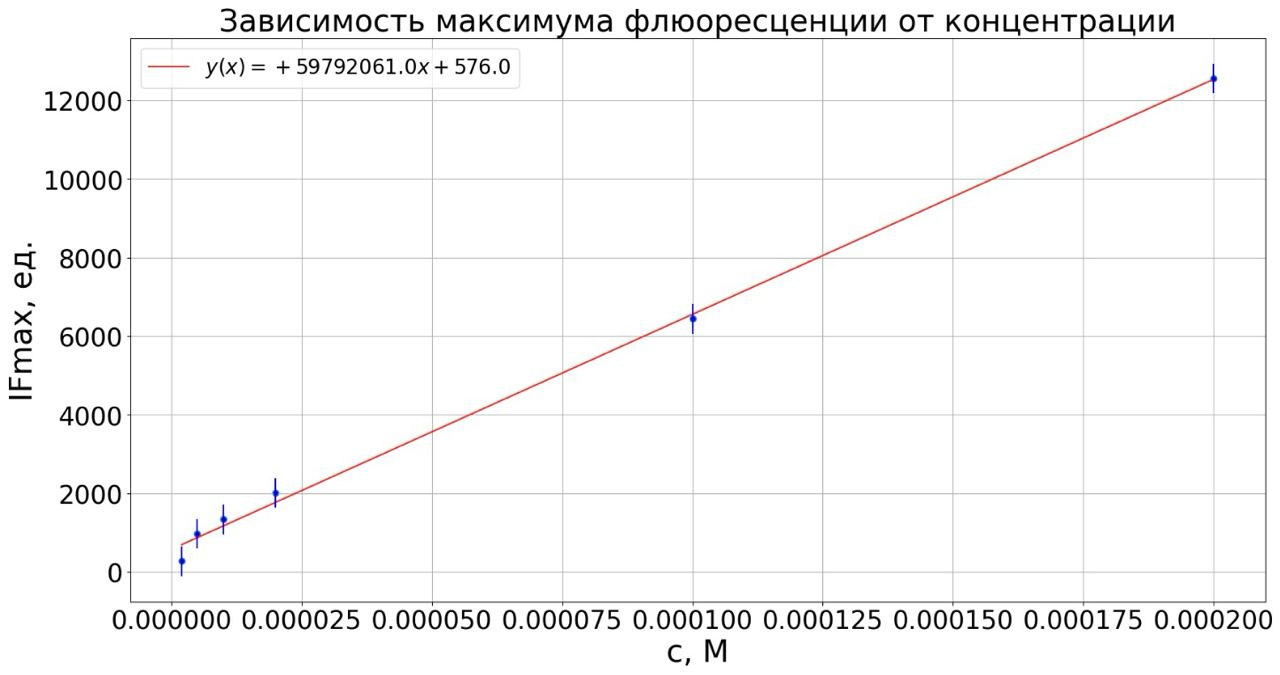
\includegraphics[scale=0.3]{photo_2024-04-16 23.48.43.jpeg}}
\caption{Зависимость максимума флуоресценции от концентрации}
\end{figure}

\item Снимем спектры поглощения растворов родамина 6G различной концентрации. Наблюдаем зависимость максимума пика от концентрации раствора при длине волны примерно 500-550 нм.
\begin{figure}[h!]
\center{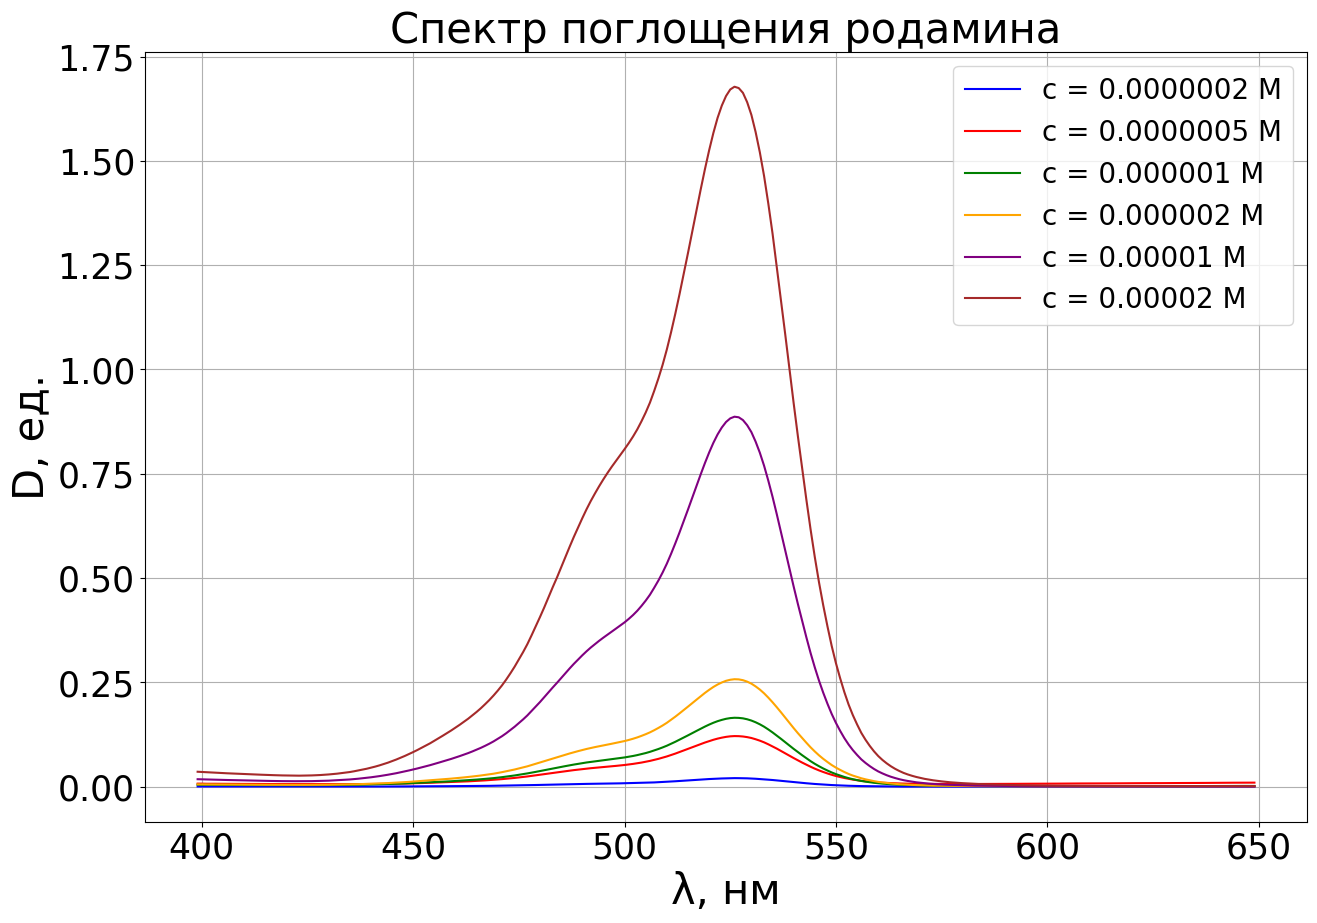
\includegraphics[scale=0.3]{pogl_ne_norm.png}}
\caption{Поглощение родамина 6G в зависимости от его концентрации}
\end{figure}

Построим график зависимости максимума поглощения от концентрации раствора. Зависимость хорошо описывается линейной функцией. По графику можно оценить коэффициент молярной экстинкции: $$D = log_{10}(I_0/I)=\varepsilon l C$$
$$\varepsilon = \frac{D}{lc} = 8100 \pm 300 \frac{1}{\text{см М}} $$


\begin{figure}[h!]
\center{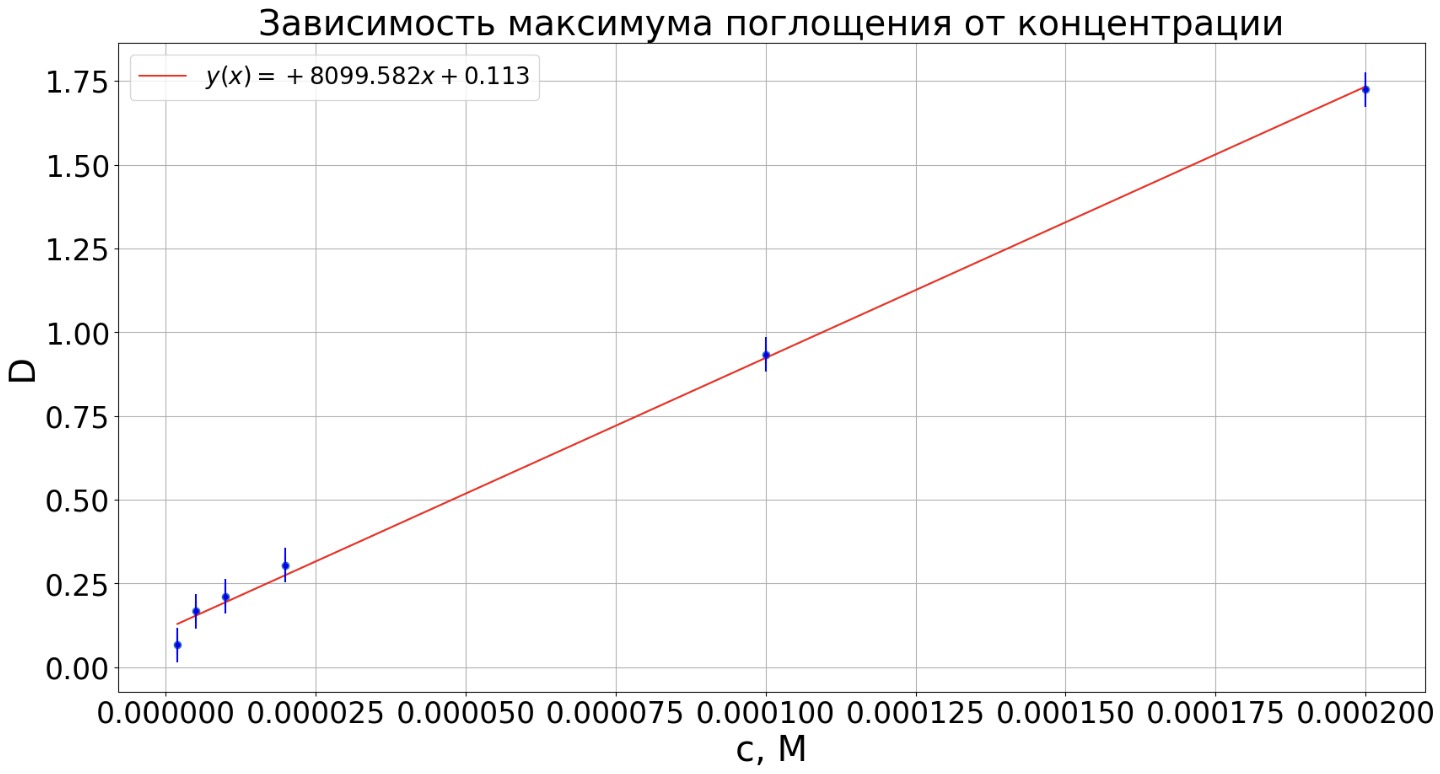
\includegraphics[scale=0.3]{tg_image_1586412095.jpeg}}
\caption{Зависимость максимума поглощения от концентрации
}
\end{figure}

    \subsection*{Задание 2. Исследование тушения флуоресценции родамина 6G йодид-ионами}
\item Приготовим серию растворов родамина 6G в концентрации $5 \cdot 10^{-6}$ М и KI различных концентраций. Построим спектры флуоресцентции раствора родамина 6G для всех концентраций тушителя. 

\begin{figure}[h!]
\center{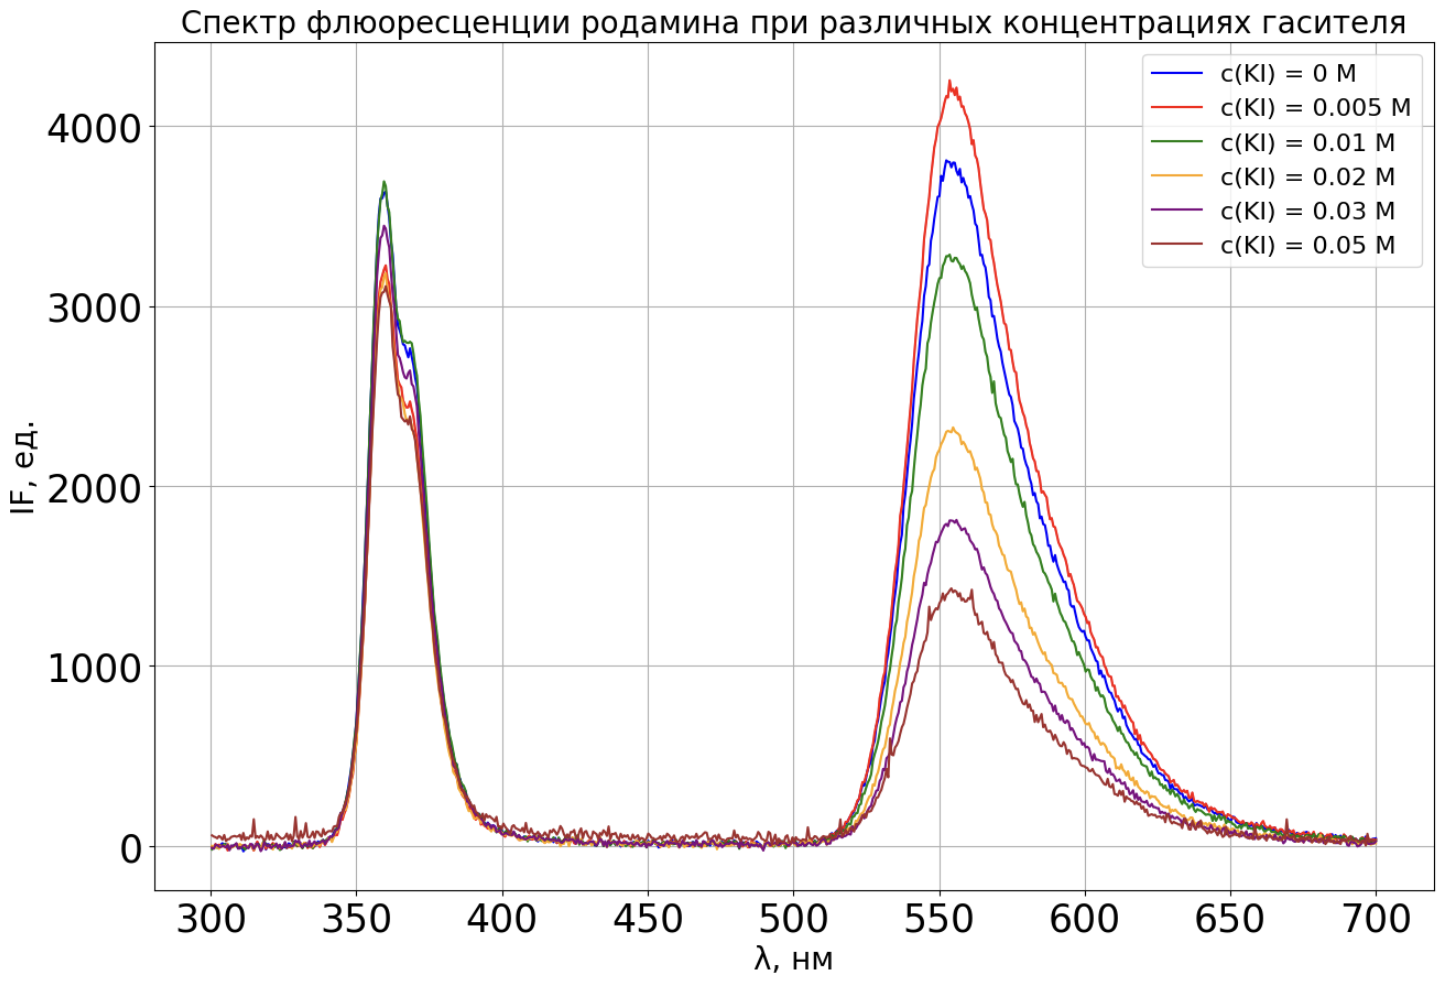
\includegraphics[scale=0.55]{Screenshot 2024-04-16 at 23.54.12.png}}
\caption{Спектры флуоресценции от концентрации KI}
\end{figure}

Построим зависимость интенсивности флуоресценции $F$ от концентрации KI. 

Построим зависимость $F_0/F$ от концентрации KI, где $F_0$ - интенсивность флуоресценции чистого раствора родамина.
\begin{figure}[h!]
\center{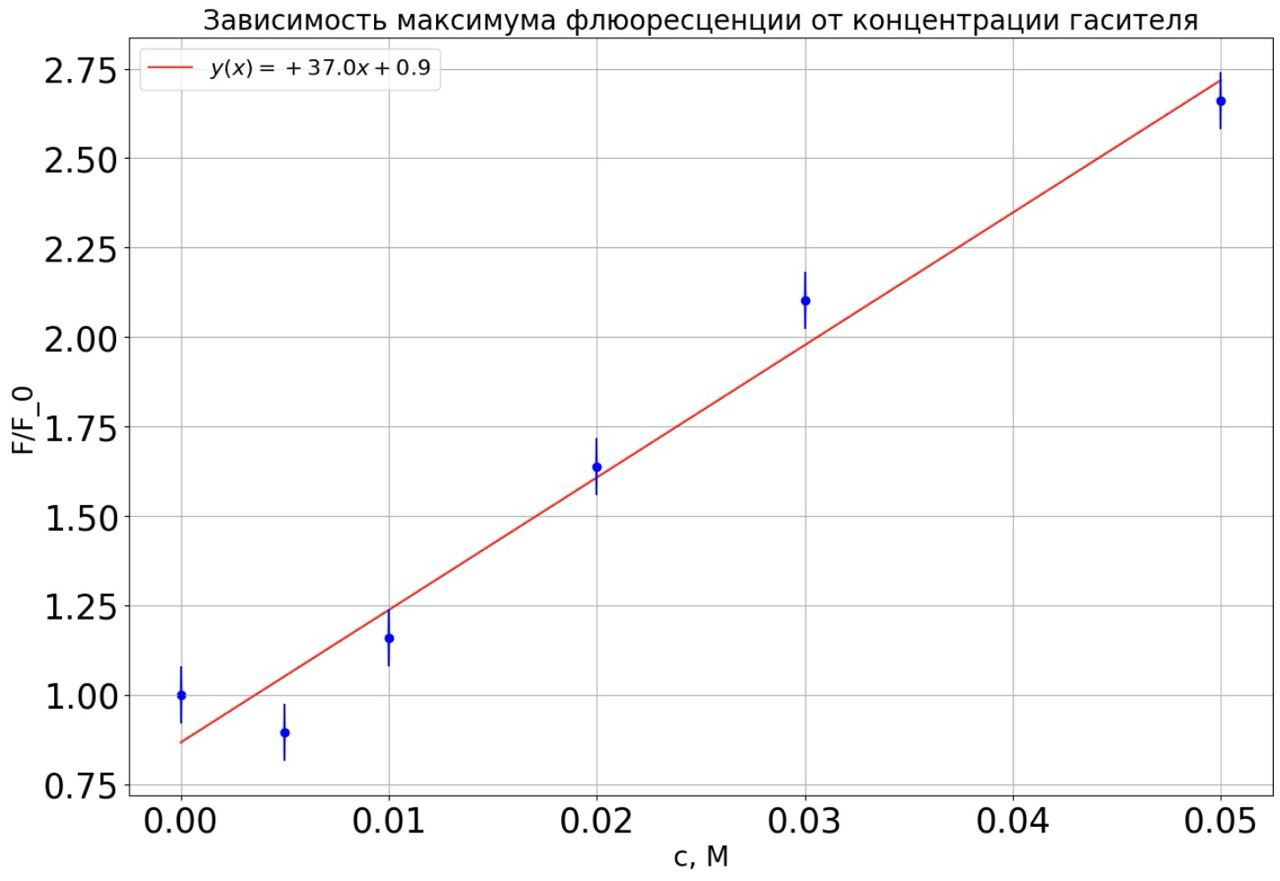
\includegraphics[scale=0.3]{gasitel_fluor.jpeg}}
\caption{Зависимость интенсивности флуоресценции от концентрации KI}
\end{figure}


Штерн-фольмеровская константа тушения была получена из наклона графиков зависимости $F_o/F$ от концентрации тушителя:
\begin{equation}
   K_{\text{дин}} = (37 \pm 4) \frac{1}{M}
\end{equation}

\begin{equation}
   K_{q} = \frac{K_{\text{дин}}}{\tau_0} = (0.37 \pm 0.04) \cdot 10^{10} \frac{1}{M c}
\end{equation}

Диффузионно-контролируемая бимолекулярная константа скорости $K_0$ может быть вычислена по уравнению Смолуховского:

\begin{equation}
   K_0 = 4 \pi R_{\sum} D_{\sum} N_A.
\end{equation}

где радиус молекулы может быть вычислен с помощью формулы для молярной массы:
\begin{equation}
   R_{i} = \sqrt[3]{\frac{M_i}{4 \pi \rho_i N_A}}
\end{equation}

коэффициент диффузии:

\begin{equation}
   D = \frac{kT}{6 \pi \rho \eta}
\end{equation}

Таким образом, бимолекулярная константа скорости $K_0$:

\begin{equation}
   K_0 = 4 \pi (R_1 + R_2) N_A \frac{kT}{6 \pi \rho \eta} \frac{(
R_1+R_2)}{R_1 R_2} = 9009 \frac{1}{\text{М с}}.
\end{equation}

Тогда эффективность тушения:

\begin{equation}
       w = \frac{K_q}{K_0} = (41 \pm 4) \cdot 10^4

\end{equation}

\end{enumerate}


\section*{Выводы}
\begin{itemize}
    \item В данной работе мы получили спектры флуоресценции водных растворов родамина 6G различных концентраций. Зависимость максимумов интенсивности от концентрации оказалась линейной. При увеличении концентрации сигнал флуоресценции увеличивается, это объясняется увеличением числа излучающих молекул. 
    \item Мы получили спектры поглощения растворов родамина 6G различной концентрации. Предполагая справедливость закона Бугера-Ламберта-Бера, мы получили коэффициент молярной экстинкции: $\varepsilon = 8100 \pm 300 \frac{1}{\text{см М}}$. Теоретическое значение составляет $\varepsilon = 10^4 \frac{1}{\text{см М}}$. По порядку величины значения совпали.
    \item Мы исследовали зависимость тушения флуоресценции родамина 6G йодид ионами. При увеличении концентрации тушителя значительно падала интенсивность флуоресценции. Зависимость отношения интенсивности описывается законом Штерна-Фольмера. Эффективность тушения оказалась: $w = (41 \pm 4) \cdot 10^4$
\end{itemize}

\end{document}

